\documentclass[10pt]{article}
\usepackage{url}
\usepackage{cbic2011}
\usepackage{times,amsfonts,enumerate,amssymb,amsmath,epsfig,bm,cite}
\usepackage{color}
\usepackage[utf8]{inputenc}
\usepackage[OT1]{fontenc}
\usepackage[brazil]{babel}
\usepackage{float}

%%%%%%%%%%%%%%%%%%%%%%%%%%%%%%%%%%%%%%%
%%% Definicao das dimensoes da pagina

\usepackage[a4paper,
hmargin={2cm,1cm},
vmargin={2cm,2cm},
footskip=5mm]{geometry}

%%%%%%%%%%%%%%%%%%%%%%%%%%%%%%%%%%%%%%%

\hyphenation{IEEE}

\newcommand\mf[1]{\text{\boldmath$#1$}}

\begin{document}

\title{
    De Volta ao Ponto: Uma abordagem prática para re-alinhamento de \textit{backlogs}\\ \smallskip
    \small{TRABALHO DE CONCLUSÃO DE CURSO}
}

\author{
 	{\bf Diego dos Santos Centeno }\\ 
 	{\normalsize Pós-Graduação em Tecnologias Aplicadas a Sistemas de Informação com Métodos Ágeis} \\
 	{\normalsize Centro Universitário Ritter Dos Reis - UNIRITTER} \\
 	{\normalsize centeno@diegocenteno.com}  \\ \\
	%
 	{\bf Émerson Barbiero Hernandez} \\
 	{\normalsize Professor Orientador}\\
 	{\normalsize emerson.hernandez@gmail.com} \\
}
\maketitle


\begin{abstract}
\maketitle
\noindent
\small
Uma Concepção (em inglês, Inception) é uma dinâmica com foco na descoberta do produto, aplicada a projetos de software. Esta atividade visa promover um maior alinhamento entre o time de desenvolvimento e o cliente em relação ao conceito do produto e as expetativas gerais. O objetivo de uma Concepção é preparar o time envolvido para um desenvolvimento inteligente e ágil do produto proposto, reduzindo o risco de conflitos de expectativas e retrabalho. O resultado desses experimentos é ter uma equipe alinhada quanto às necessidades e prioridades que o desenvolvimento do produto requer no curto, médio e longo prazo.
Porém o mundo se move rápido e as necessidades de negócio mudam o tempo todo, então é preciso constantemente verificar se o planejamento existente atende as expectativas de negócio ou se precisamos modificar o planejado para se adaptar as novas necessidades do mercado.
Neste trabalho vamos apresentar uma abordagem pratica de Concepção Enxuta (em inglês, Lean Inception) que foca no alinhamento e validação de um \textit{backlog} existente através de um conjunto de dinâmicas e metodologias já existentes, porém já testadas e validadas em um ambiente real.

\noindent
%PALAVRAS-CHAVE} 
\textbf{Palavras-chave}: Metodologia ágil, Concepção Enxuta, Lean.
\end{abstract}

\maketitle
\section{Introdução}\label{sec:introducao}
    As metodologias ágeis têm sido cada vez mais apontadas como a melhor alternativa para o desenvolvimento de software. O termo 'ágil' refere-se a uma filosofia de desenvolvimento de software. Elas propõem uma nova abordagem de desenvolvimento, eliminando gastos com documentação excessiva e burocrática, enfatizando a interação entre pessoas e nas atividades que efetivamente trazem valor e produzem software com qualidade\cite{Agilmanifesto}. Podemos também dizer que a aplicação das metodologias ágeis no desenvolvimento de software, ou simplesmente desenvolvimento ágil de software, é o desenvolvimento iterativo e incremental onde as hipóteses (ou requisitos) são testadas e implementadas por colaboração entre pequenos times auto-organizados e multifuncionais.\cite{Bastos:Luca} Debaixo deste amplo guarda-chuva estão abordagens mais específicas como Extreme Programming (XP), Scrum e Desenvolvimento Enxuto (Lean). Cada uma dessas abordagens em particular possui suas próprias ideias, comunidades e líderes.\cite{Fowler:NewMethodology}

    Dentro deste novo paradigma uma prática muito emergente é criar colaborativamente o entendimento sobre o produto a ser desenvolvido antes de sair simplesmente programando. Diferentes abordagens têm sido propostas para que os times descubram e entendam coletivamente o escopo se ser desenvolvido, dentre elas a mais comum é a Concepção (em inglês, Inception).
    
    Diante das várias possibilidades de formatos de se fazer uma concepção, uma que vem se destacando em número de adeptos e projetos é a Concepção Enxuta (Lean Inception), também conhecida como Direto ao Ponto.\cite{Caroli:DiretoAoPonto} Ela consiste em um conjunto de atividades com a finalidade de clarear e alinhar o objetivo do produto, aprofundar para quem é este produto e como esse usuário interage com ele, assim pensando em suas funcionalidades e após faz um sequenciamento dessas funcionalidades para determinar qual o mínimo produto viável.

    No entanto, devido a complexidade de um projeto e as todas as tarefas do dia-a-dia, perdemos de vista aquilo que queremos alcançar. Dada a natureza do trabalho colaborativo, juntamente com os pontos citados anteriormente, é necessário de tempos em tempos realinhar o escopo das funcionalidades inicialmente pensadas na Inception. Com isto precisamos voltar ao planejamento inicial, ou seja, precisamos voltar ao Direto ao Ponto. Este artigo apresenta uma abordagem prática do uso de dinâmicas para re-validar e re-alinhar as funcionalidades e MVPs que surgiram na Inception Enxuta, chamado de "De Volta ao Ponto".


\section{Revisão de Literatura}\label{sec:literatura}
    \subsection{\textit{Design Thinking}}\label{subsec:literatura-design-think}
        O \textit{Design Thinking} é um processo colaborativo de pensamento crítico e criativo que permite organizar informações e ideias, para tomar decisões, aprimorar situações e adquirir conhecimento \cite{DesignThink:Vianna}. Sendo assim, pode-se dizer que ele é um método que trabalha essencialmente a cocriação e utiliza algumas práticas valiosas de descoberta. Desta forma, e até mesmo por possibilitar a coleta de resultados imediatos a partir de ações simples, acaba por auxiliar também no aculturamento da empresa.
        O \textit{Design Thinking} é um método bastante eficaz e presente nas organizações que buscam realmente entender, avaliar e implementar o que os seus clientes e/ou \textit{stakeholders} pensam sobre seus produtos e serviços. A sua utilização abrange diferentes ramos da indústria, podendo ser considerada também uma ferramenta estratégica que incentiva a criação conjunta a partir de uma visão por processos. E nesta perspectiva, o processo de Design Thinking é definido, conforme as seguintes fases \cite{DesignThink:Vianna}:
        
        \begin{itemize}
            \item \textbf{Imersão} (entendimento) - envolve a contextualização do projeto;
            \item \textbf{Ideação} (criação) - tem o intuito de gerar ideias inovadoras para o tema de projeto;
            \item \textbf{Prototipação} (teste) - tem como função validar hipóteses a partir da formulação de questões, criação de protótipos, testes, avaliações e conclusão;
            \item \textbf{Desenvolvimento} (aplicação) - o próprio uso do conhecimento adquirido através do processo criativo.
        \end{itemize}
        
    \subsection{Desenvolvimento Enxuto}\label{subsec:literatura-lean}
        
        Desenvolvimento Enxuto (em inglês Lean Development) é inspirado na abordagem do mesmo nome aplicado aos sistemas de produção, que foi iniciado por Taiichi Ohno na Toyota e é também conhecido como “Sistema Toyota de Produção” \cite{Lean:Toyota} . Essa filosofia de gerenciamento de processos transformou completamente a abordagem da fabricação de automóveis, que evoluiu para um modelo mais responsável, muito mais sustentável e, ao mesmo tempo, mais eficiente.
        
        O desenvolvimento enxuto originou-se de um livro  popular de Tom e Mary Poppenieck onde foram incorporados os princípios da fabricação enxuta para o desenvolvimento de software. \cite{Lean:Poppendieck} Os seus benefícios contribuíram para a disseminação rápida desta metodologia, que agora é generalizada entre a comunidade global de métodos ágeis.
        
        Há uma série de aspectos que configuram este modelo de desenvolvimento. Sua aplicação é uma condição necessária para a existência de ajuste e, portanto, são conhecidos como os 7 princípios fundamentais do desenvolvimento de software enxuto:
        
        \begin{enumerate}
            \item \textbf{Eliminar o desperdício}: 
            Maximar o trabalho a não ser feito, seja evitando retrabalhos, processos e funcionalidades extras, defeitos, estoque de tarefas, atrasos e esperas;
            
            \item \textbf{Amplificar conhecimento}: 
                Priorizar a comunicação e o \textit{feedback} contínuos entre equipes e usuários durante o processo de desenvolvimento de software;
            \item \textbf{Adiar decisões}:
                Deixar as decisões e comprometimentos para o último momento responsável, permitindo coletar informações e ter experiências para fortalecer a tomada de decisão;
            \item \textbf{Entregas rápidas}: 
                Maximizar o retorno do investimento (\textit{ROI}) do projeto, entregando software de valor de forma rápida e contínua;
            \item \textbf{Fortalecer o time}: 
                Empoderar o time e criar um ambiente onde a equipe trabalhe de forma auto-organizada e auto-dirigida, evitando micro-gerenciamento;
            \item \textbf{Construir qualidade}: 
                Garantir qualidade no desenvolvimento do software utilizando técnicas como TDD, refatoração e integração continua;
            \item \textbf{Otimizar o todo}: 
                Entender que o software concluído é muito mais que a soma das partes entregues e verificar como ele está alinhado com os objetivos da empresa.
        \end{enumerate}
        
        
    \subsection{Concepção Enxuta}\label{subsec:literatura-inception}
        
        A Concepção Enxuta, como o próprio nome sugere, é uma abordagem mais enxuta de concepção. Esse método consiste em  um laboratório colaborativo, onde em uma semana de trabalho, o plano é compreender o objetivo do projeto, identificar os principais usuários que terão contato com a solução e o escopo funcional de alto nível, ter insumos para definição da estratégia de lançamento incremental dos \textit{MVP}s (em português, Produto Mínimo Viável). A metodologia de Concepção Enxuta é uma técnica para compreender e planejar as entregas incrementais dos MVPs. A técnica organiza as ideias e funcionalidades em um modelo que busca compreender o objetivo principal do produto, considerando as jornadas dos usuários e os incrementos de entrega.
        
        Com atividades eficazes e rápidas, a técnica desafia as considerações tradicionais de projeto, como análise de requisitos, estimativas, escopo, capacidade e planejamento detalhado. Ao longo da execução de um Concepção Enxuta devemos alcançar as seguintes etapas:
        
        \begin{itemize}
            \item Descrever a visão do produto;
            \item Priorizar os objetivos de negócio;
            \item Descrever os usuários, seus perfis e necessidades que impulsionam a funcionalidade do produto;
            \item Entender o escopo funcional de alto nível;
            \item Detalhar percepções de risco, esforço e valor de negócio por área funcional;
            \item Descrever as principais jornadas de usuários;
            \item Definir um roteiro de lançamento incremental, mostrando claramente os incrementos de \textit{MVP};
            \item Estimar esforço por amostragem;
            \item Calcular custos e especificar datas e cronograma de entrega.
        \end{itemize}
        
        
    

\section{Abordagem prática}\label{sec:abordagem}

    A abordagem apresentada aqui é, assim como no modelo de Concepção Enxuta, um \textit{workshop} colaborativo. O foco deste evento é realinhar os membros da equipe sobre o objetivo do projeto, sobre o escopo que ainda precisa ser feito e mais do que tudo sobre o caminho a seguir. Este \textit{workshop} consiste basicamente em executar uma sequência de atividades e dinâmicas, baseadas em \textit{design thinking}, para agrupar, organizar, detalhar e priorizar o trabalho e o caminho a ser seguido. Após realizarmos a concepção, saímos com uma lista de funcionalidades a serem executadas. O nome dado a esse conjuntos de funcionalidades é \textit{backlog}.
    
    Entretanto, diversos motivos inerentes da natureza do trabalho iterativo e incremental nos levam a perder de vista aquilo que realmente queremos como objetivo. Objetivo esse que foi desmembrado em diversas funcionalidades dentro do \textit{backlog}. Alguns motivos podem ser mais básicos, como por exemplo o alto nível de envolvimento da equipe nas tarefas do dia-a-dia, ou até mesmo motivos mais complexos, como por exemplo a rotatividade de membros da equipe.
    
    Por esta razão, é muito importante re-alinhar, como equipe, se o \textit{backlog} gerado anteriormente está no rumo correto para que o objetivo seja atingido. Fazendo isto podemos, no mínimo, ter alguns ganhos para o produto/projeto ou até mesmo para a organização:
    \begin{itemize}
        \item \textbf{Validar o que já foi feito}: Validar se as hipóteses imaginadas e as funcionalidades já desenvolvidas efetivamente atenderam as necessidades do produto/projeto;
        \item \textbf{Revalidar o caminho a seguir}: Projetos assumem um caminho a seguir, mas, na prática o caminho é mais distorcido do que planejamos; esta dinâmica ajuda a revalidar o caminho, subindo e baixando de nível, considerando o conhecimento atual e o objetivo a alcançar;
        \item \textbf{Gerar entendimento compartilhado}: É sempre importante que o objetivo e o contexto do que precisa ser feito seja de conhecimento de todos os membros da equipe;
        \item \textbf{Reduzir \textit{ramp-up} do \textit{onboarding}}: este realinhamento do \textit{backlog} pode ser aproveitado para gerar contexto para quem está entrando no time, diminuindo assim a curva de aprendizado para quem está entrando;
        \item \textbf{Reduzir riscos}: Quanto mais vezes checamos se estamos alinhados e caminhando em direção ao objetivo, menos riscos corremos de não atingir ou até mesmo fugir do objetivo.
    \end{itemize}
    

    	\subsection{Definindo os objetivos}\label{sec:abordagem-objetivos}
            Primeiro é necessário subir de nível, deixar o \textit{backlog} um pouco de lado, e entender os objetivos do projeto ou da equipe. Para isto, utilizamos a técnica do 'Diamante duplo'\cite{DoubleDiamond}, em sua primeira parte: Descobrir e Definir. O primeiro diamante, conforme apresentado na figura~\ref{figura:1}, sugere que inicialmente deve-se gerar opções a fim de encontrar novas possibilidades e a partir dele, gerar opções.
            
            \begin{figure}[H]
        		\centering
        		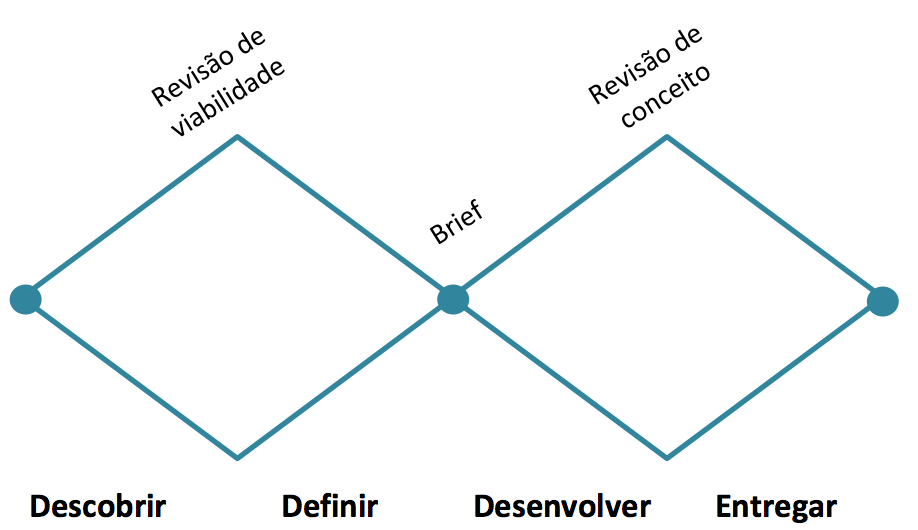
\includegraphics[width=.5\textwidth]{images/diamante-duplo.png}
        		\caption{Diamante Duplo}
        		\label{figura:1}
        	\end{figure}
        	
            Primeiramente, abrimos espaço para que uma série de ideias sejam descobertas e compartilhadas entre os membros da equipe. Normalmente fazemos isso com o formato de um \textit{brainstorm}. Esse o momento de divergir e descobrir. O objetivo não é criar uma lógica racional ou traçar um caminho de solução para o problema, procura-se gerar o maior número de alternativas e contextos possíveis e a partir disso, decidir qual são as melhores opções. Feito isto, é momento de convergir e definir. Nesta segunda etapa deve-se discutir com a equipe os objetivos levantados a fim de identificar quais são potencialmente semelhantes e então agrupá-los. Devemos sair desta etapa com no máximo 5 objetivos por três simples motivos:
            \begin{itemize}
                \item \textbf{Foco}: Ter muitos objetivos pode fazer com desviemos o foco ao longo do caminho, com isso podemos acabar não atingindo nenhum deles.
                \item \textbf{Validação}: Manter o foco em poucos objetivos vai fazer com que o time seja capaz de rodar periodicamente esta dinâmica para revalidar os mesmos. 
            \end{itemize}
        
        \subsection{Aplicando OKRs}\label{sec:abordagem-como-okr}
            
            De posse dos objetivos identificados na atividade anterior(~\ref{sec:abordagem-objetivos}), agora é a vez de utilizarmos a metodologia de \textit{OKRs} para estabelecer o caminho para atingirmos os mesmos. A metodologia OKR (Objectives and Key Results) nasceu dentro da Intel, no Vale do Silício, com a missão de estabelecer objetivos e resultados-chave para mensurar o quão próximo se está do objetivo. Essa metodologia vem sendo adotada desde a década de 90 em vários empreendimentos, independente de tamanho, desde grandes corporações até startups.\cite{OKR:Castro-1} Na metodologia OKR, primeiro você cria um objetivo e, em seguida, configura um conjunto de resultados chave:\cite{OKR:Castro-2}: 
            \begin{enumerate}
                \item \textbf{Objetivos} (\textit Objective): É uma descrição qualitativa do que deseja alcançar. Os objetivos devem ser curtos, inspiradores e envolventes. Um Objetivo deve motivar e desafiar a equipe.
                \item \textbf{Resultados chave} (\textit Key Results): São um conjunto de métricas que medem o seu progresso e o impacto direto no atingimento do objetivo, caso seja realizada com sucesso. Para cada Objetivo, você deve ter um conjunto de 2 a 5 resultados chave.
            \end{enumerate}
                
            John Doerr, idealizador da metodologia na Intel e também responsável por sua implementação no Google, criou um modelo bastante simples de aplicação de  \textit{OKRs}:\cite{OKR:John}
            \begin{quote}
            \centering
                \textbf{Eu vou} \underline{ objetivo } \textbf{mensurado por} \underline{ lista de resultados chave}
            \end{quote}
            
            Utilizando o modelo acima, devemos criar de 3 a 5 resultados chave para cada objetivo. O conjuntos destes resultados chave é, para nós, o balizador para saber se atingimos o objetivo ou não. Ao final desta atividade, devemos ter uma lista que se assemelha a figura~\ref{figura:2}.
            
            \begin{figure}[H]
        		\centering
        		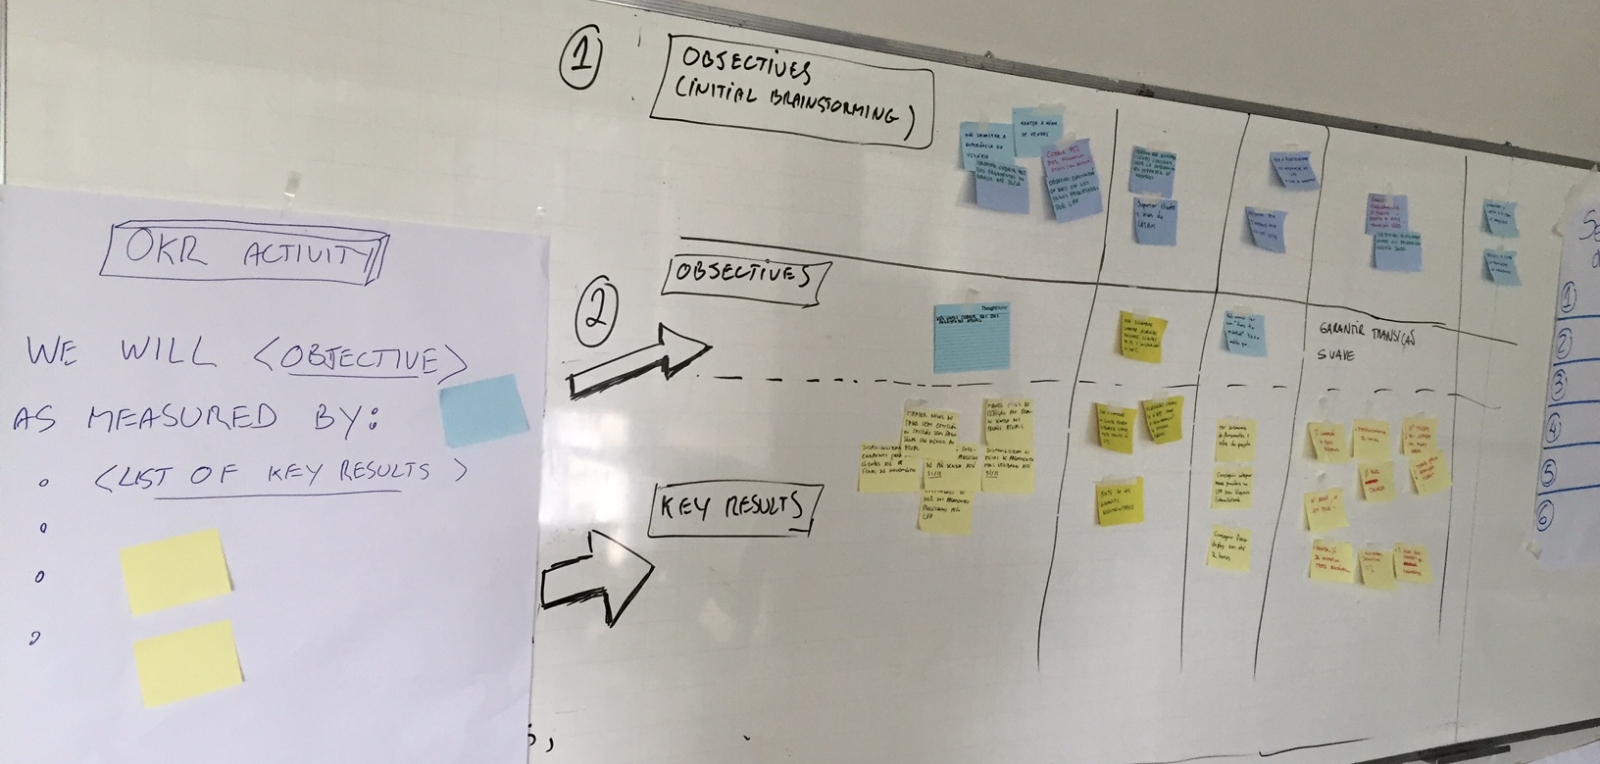
\includegraphics[width=.7\textwidth]{images/como-okr.png}
        		\caption{Exemplo de como aplicar o modelo de \textit{OKRs}}
        		\label{figura:2}
        	\end{figure}
            
        
        \subsection{\textit{Backlog}}\label{sec:abordagem-como-backlog}
            A partir desta etapa, vamos passar a trabalhar exclusivamente com o nosso \textit{backlog}. A ideia é entrar nessa atividade com o \textit{backlog} atual e, ao final da abordagem, sair com um novo \textit{backlog} (seja por incluir novas funcionalidades, cortar algumas que não fazem mais sentido ou até mesmo pelo simples fato de re-priorizar o mesmo).
            
            A primeira coisa a ser feita é listar todo o \textit{backlog} atual e garantir que todos os itens desta lista estão no mesmo nível de abstração. Durante as dinâmicas que vamos aplicar estaremos trabalhando sempre a nível de funcionalidades, mas podem também ser trabalhado em qualquer nível abstração, como estórias, épicos ou até mesmo tarefas. Neste momento não há necessidade alguma de vincular os itens do \textit{backlog} com a pratica de \textit{OKR} que fizemos anteriormente, afinal de contas, indiretamente, vamos estar olhando para as funcionalidade já com a visão que definimos na dinâmica anterior.

        \subsection{Método da cebola}\label{sec:abordagem-como-cebola}
            De posse da lista de funcionalidades (histórias ou épicos), é o momento de identificarmos e validarmos o quanto destas funcionalidades já foram implementadas. Existem diversas formas de fazer isto, porém aqui vamos utilizar uma dinâmica criada pelo Lourenço Soares.\cite{Lourenco:Cebola}
            
            Inicialmente o método da cebola foi criado e utilizado para escrever as histórias de uma funcionalidade e ou épico. Ele consiste idealmente em ir descrevendo as histórias em camadas, ou seja, coloca-se a tarefa mais básica no núcleo da cebola, após se cria uma camada em volta deste centro e se coloca as tarefas um pouco mais complexas. Repete-se isto até que todas as tarefas da história sejam mapeadas, como pode ser visto na figura ~\ref{figura:3}. 
            
            Como já temos as nossas histórias prontas e o que buscamos é identificar quanto destas funcionalidades já foram implementadas, iremos utilizar o método da cebola de uma forma um pouco distinta. Iremos utilizar conceito de camadas do método da cebola para validar o quanto já avançamos com a funcionalidade e, para isto, vamos utilizar apenas três camadas (vide figura ~\ref{figura:3}). A ideia aqui é que, para cada história, possamos saber o quanto já foi concluído e assim atribuirmos a história uma \textit{tag}:
            \begin{itemize}
                \item \textbf{R1}: significa que tudo ou muito ainda precisa ser feito
                \item \textbf{R2}: significa que já avançamos bastante, porém ainda dá algumas coisas para serem feitas
                \item \textbf{R3}: significa que já estos muito próximos de terminar
            \end{itemize}
            
            É comum que neste momento a equipe se dê por conta que determinada funcionalidade já foi implementada em uma outra história ou até mesmo que essa funcionalidade não faz mais sentido para o projeto, produto ou para a própria equipe.
            
            \begin{figure}[H]
        		\centering
        		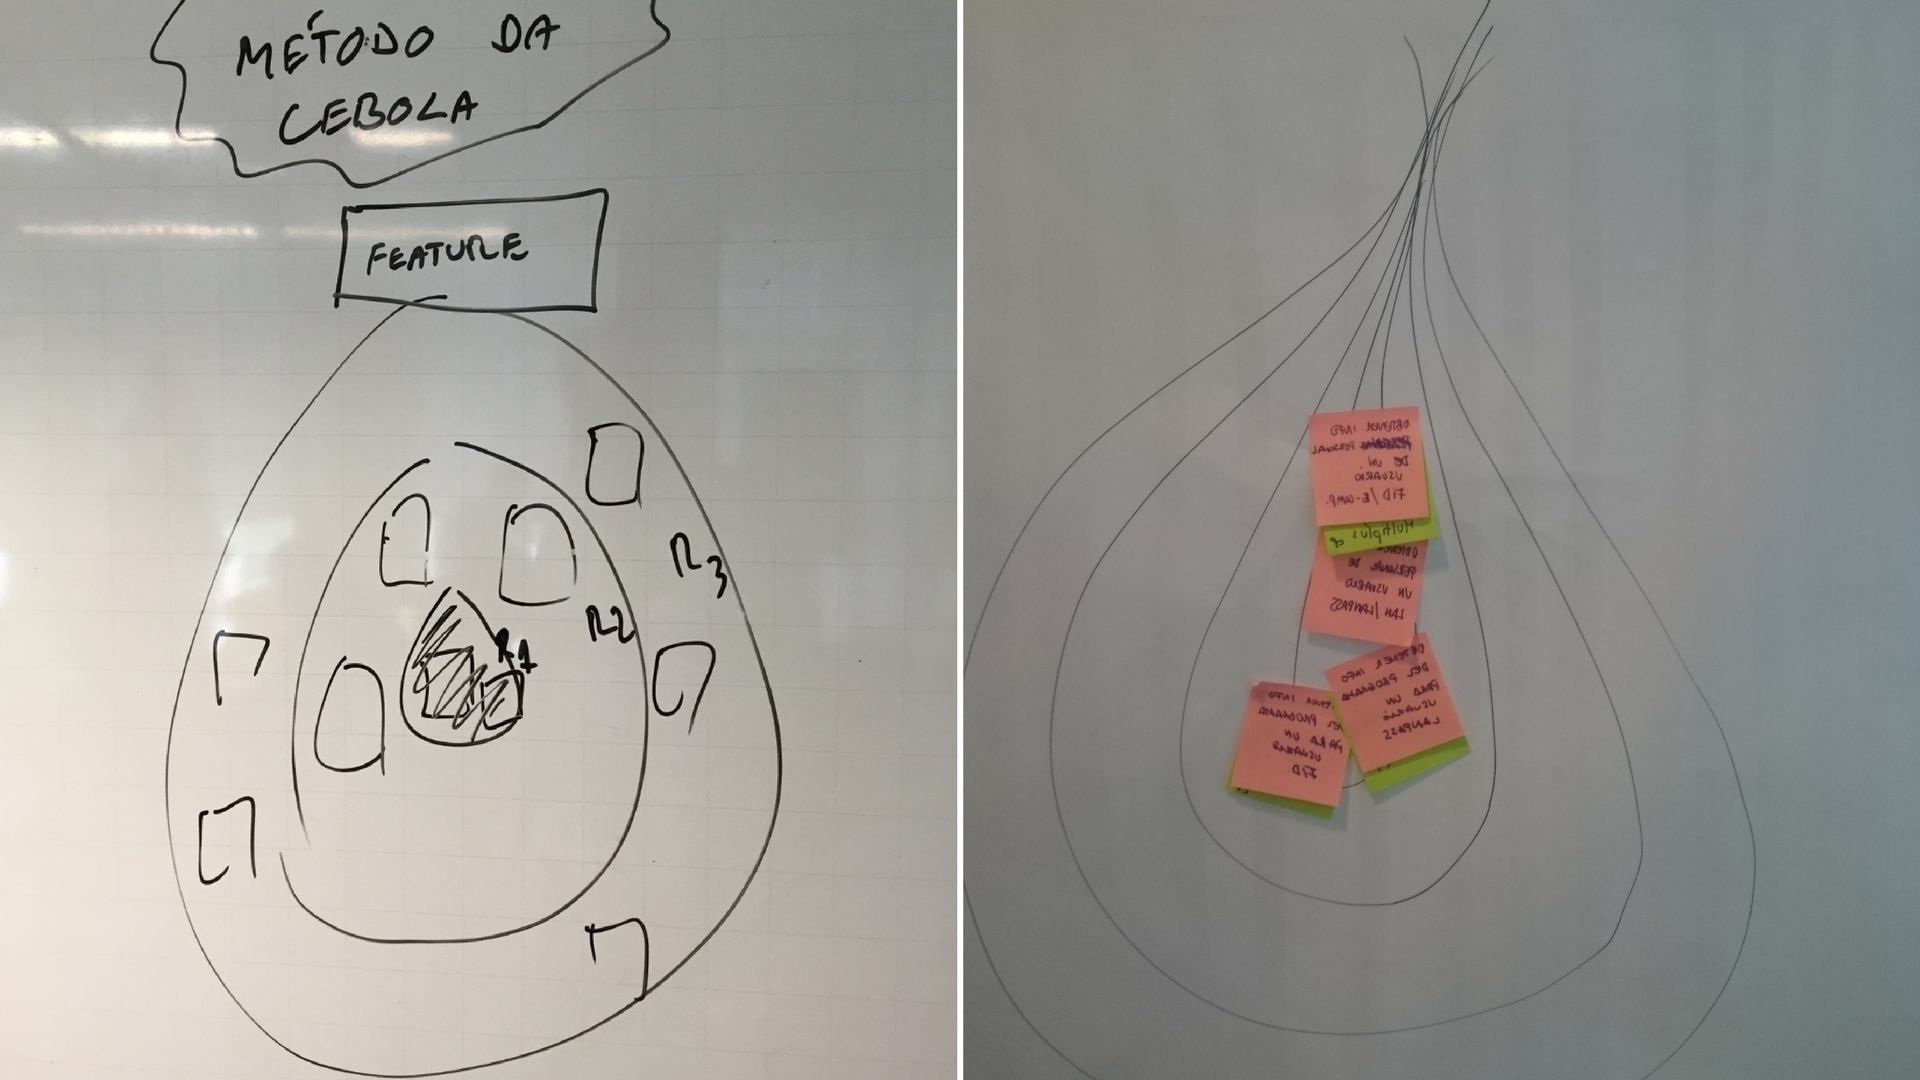
\includegraphics[width=.7\textwidth]{images/como-cebola.png}
        		\caption{ Exemplo do método da cebola / Exemplo de aplicação do método da cebola}
        		\label{figura:3}
        	\end{figure}
        
        \subsection{\textit{Canvas} de esforço versus valor de negócio}\label{sec:abordagem-como-valor-esforco}
            Uma vez que já conhecemos o nosso \textit{backlog} e identificamos o quanto já avançamos com as funcionalidades, agora é hora de identificar o nível de esforço e o valor de negócio associado a cada funcionalidade. Faremos isso seguindo os passos sugeridos pelo Paulo Caroli no livro \textit{Direto Ao Ponto} \cite{Caroli:DiretoAoPonto}:
            
            \begin{enumerate}
                \item Vamos criar um \textit{canvas} (gráfico) com dois eixos, onde o eixo X vai representar o esforço (a dificuldade e o trabalho que será necessário para completar tal funcionalidade) e o eixo Y vai representar o valor para o negócio desta funcionalidade.
                
                Também iremos criar uma escala para um dos eixos (conforme figura ~\ref{figura:5}), no eixo de esforço vamos adotar: \textit{E}, \textit{EE} e \textit{EEE} (onde \textit{E} representa um baixo esforço e \textit{EEE} representa um alto esforço), no eixo de valor de negócio vamos adotar: \textit{\$}, \textit{\$\$} e \textit{\$\$\$} (onde \textit{\$} representa um baixo esforço e \textit{\$\$\$} representa um alto esforço). 
                
                \begin{figure}[H]
            		\centering
            		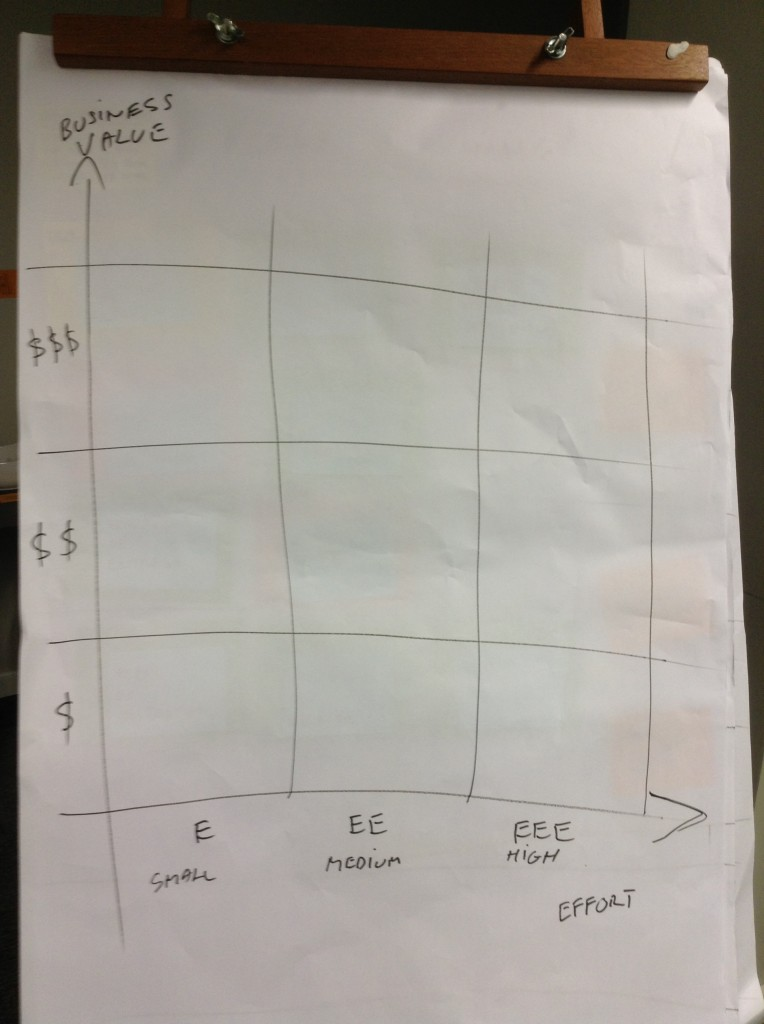
\includegraphics[width=.4\textwidth]{images/canvas-esforco-valor.jpg}
            		\caption{\textit{Canvas} de esforço versus valor de negócio}
            		\label{figura:5}
            	\end{figure}
                
                \item Agora vamos pegar uma funcionalidade do nosso \textit{backlog} e vamos posicionar no \textit{canvas} de acordo com o entendimento que o time tem sobre o esforço e o valor da mesma. Neste momento é importante levar em consideração a estimativa que fizemos no através do método da cebola (~\ref{sec:abordagem-como-cebola}), pois ela pode impactar diretamente na estimativa de esforço.
                
                Neste momento é importante que toda equipe partilhe da mesma opinião. Se algum membro do time não concordar com a escala aplicada, o time deve discutir os requisitos e a tecnologia envolvida de forma que haja um consenso sobre a escala da funcionalidade.
                
                \item Uma vez classificada a funcionalidade na escala de esforço e de valor, vamos marcar a mesma de acordo com escala de esforço (E, EE ou EEE) e de valor (\textit{\$}, \textit{\$\$} e \textit{\$\$\$}) que foi atribuída (vide figura ~\ref{figura:6}).
                
                \item Por fim, basta repetir os passos 2 e 3 até que todas as funcionalidades do \textit{backlog} possuam um esforço e um valor atribuído.
                
                \begin{figure}[H]
            		\centering
            		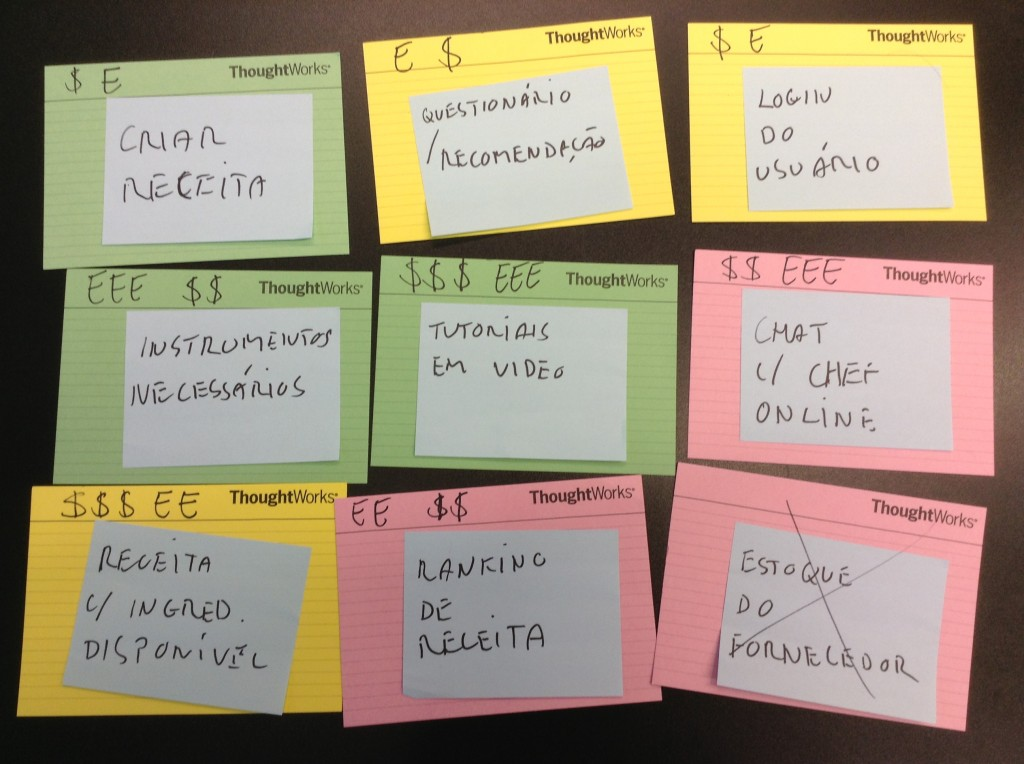
\includegraphics[width=.5\textwidth]{images/canvas-esforco-valor-2.jpg}
            		\caption{Exemplo de funcionalidade com marcações de esforço e valor}
            		\label{figura:6}
            	\end{figure}
            \end{enumerate}
        


        \subsection{Sequenciador de funcionalidades}\label{sec:abordagem-como-sequenciador}
            Dado que já sabemos os nossos objetivos (levantados através dos \textit{OKRs}) e que também já possuímos todas as funcionalidades classificas com esforço e valor, agora é o momento de priorizarmos as mesmas. Isso vai garantir que seja possível ter uma previsibilidade miníma além de destacar os \textit{milestones} e/ou ter uma previsão de atingimento dos \textit{OKRs}.
            
            O sequenciado de funcionalidades, assim como o \textit{canvas} de esforço e valor, é um gráfico (\textit{canvas}). Porém ao invés de ser divido em blocos, ele é dividido apenas em linhas, o que aqui vamos chamar de ondas (vide figura ~\ref{figura:7}).
            
            \begin{figure}[H]
        		\centering
        		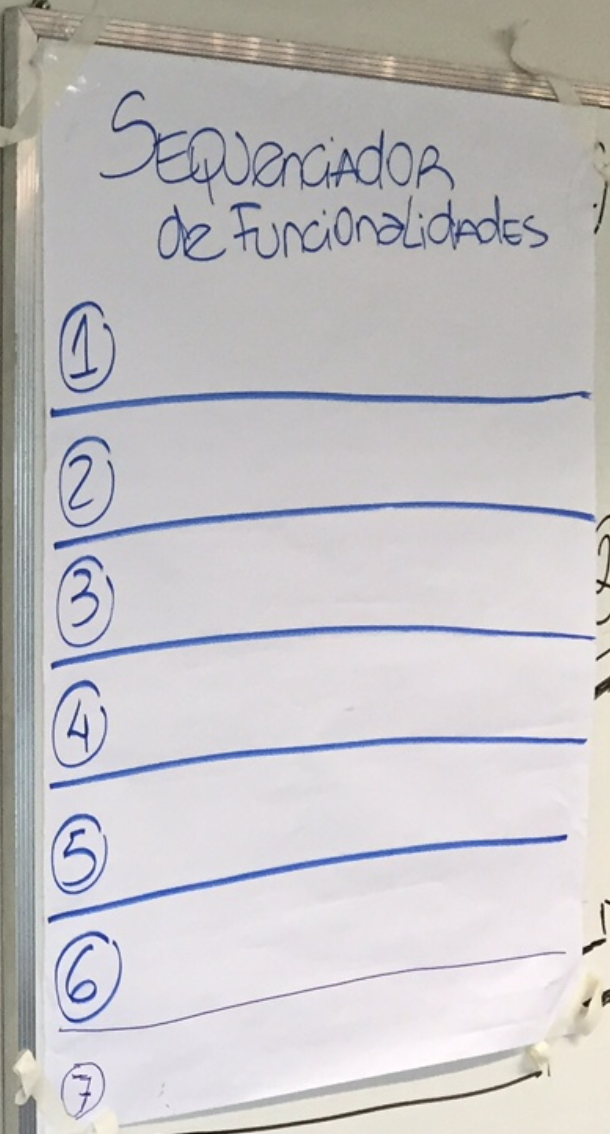
\includegraphics[width=.4\textwidth]{images/sequenciador.png}
        		\caption{Exemplo de sequenciador de funcionalidades}
        		\label{figura:7}
        	\end{figure}
        	
        	Agora é o momento do time, em conjunto, decidir e organizar a sequencia de execução das funcionalidades. O time se organizar e distribuir as funcionalidades
        	dentre as ondas, onde a primeira onda vai conter as funcionalidades que o time quer entregar primeiro e assim sucessivamente até a ultima onda.
        	
        	
        	Neste momento é importante levar em consideração as estimativas de esforço e valor que fizemos no através do \textit{canvas} de esforço versus valor (~\ref{sec:abordagem-como-valor-esforco}). Além disto é muito importante seguir algumas regras para o sequenciador seja mais efetivo:
        	
        	\begin{enumerate}
                \item Uma onda pode conter no máximo 3 funcionalidades.
                
                \item A soma de esforço das funcionalidades não pode ultrapassar 5 \textit{E}s.
                
                \item A soma de valor de negocio das funcionalidades não pode ser menos de 4 \textit{\$}s.
                
                \item Uma onda tem de conter no mínimo 2 funcionalidades.
            \end{enumerate}
        	
        	
        	As regras acima visão limitar o número de funcionalidades que serão trabalhadas ao mesmo tempo em cada onda (regra 1), evitam um período de trabalho desequilibrado com muita incerteza ou muito esforço (regra 2) e garantem um foco constante na maior entrega de valor para o negócio (regra 3 e 4).
            
\section{Considerações finais}\label{sec:consideracoes}

    O desenvolvimento do presente trabalho possibilitou uma análise de como as metodologias de Concepção Enxuta podem melhorar os resultados do processo de desenvolvimento de software ágil. Além disso, também permitiu evidenciar que não é necessário ficar preso as grandes metodologias e/ou processos de criação, ou seja, podemos adotar ou até mesmo criar dinâmicas que mais se adéquem as nossas necessidades.
    
    Durante a criação deste trabalho tivemos a oportunidade de rodar a prática descrita na seção~\ref{sec:abordagem} e assim evidenciar de forma mais consistente os ganhos aqui propostos. Rodamos a prática em 6 projetos, dos quais 3 já haviam passado pelo método \cite{Caroli:DiretoAoPonto} e tinham sua visão de produto e seus \textit{backlogs} muito bem alinhados, e outros 3 projetos que não fizeram nenhum tipo de Concepção e que apenas tinham como \textit{backlog} uma lista de funcionalidades que foram criadas a partir do projeto em andamento.
    
    O maior ganho evidenciado é a geração colaborativa de conhecimento do produto, o que reflete a curto e médio prazo na qualidade, acuracidade das entregas do produto, o que tende a impactar diretamente na diminuição dos riscos e na redução dos custos do projeto. Também foi possível observar que nos times que rodaram a prática, conseguimos atingir os seguintes resultados:
    \begin{itemize}
        \item Refinar e /ou corrigir erros de previsibilidade (estimativas) por já conhecer mais do contexto do produto/projeto;
        \item Simplificar coisas e processos dado o conhecimento adquirido durante o desenvolvimento prévio;
        \item Reconhecer que as tecnologias envolvidas evoluíram e que é possível adotar ou escolher novas alternativas;
        \item Criar mais foco nas funcionalidades faltantes, dado ao fato de construir uma visão mais unificada do que ainda falta;
        \item Guiar o desenvolvimento e as prioridades do \textit{backlog} orientado aos objetivos do produto/projeto;
        \item Criar uma fator motivacional extra através do fortalecimento e alinhamento do time, uma vez que estão todos juntos fazendo a dinâmica;
        \item Criar uma visão unificada do time sobre os objetivos do produto/projeto, sobre tudo em times que tiveram alterações de seus membros;
        \item Re-priorizar funcionalidades que já não são mais tão importantes dados os objetivos do produto/projeto.
    \end{itemize}
        
    Por se tratar de uma prática de exploração mais do que uma técnica exata aliado ao número ainda pequeno de execuções não permitiu obter dados (números e/ou indicadores) mais consistentes sobre os ganhos da aplicação da metodologia. Uma pesquisa mais aprofundada para obter dados mais consistentes sobre os ganhos de outras metodologias de Concepção e Concepção Enxuta foi realizada, mas atualmente existem poucos dados acessíveis que evidenciem o ganho direto desta metodologias.

    Deve-se levar em consideração que, apesar de ter muitas referencias diretas ao método \textit{Direto Ao Ponto} \cite{Caroli:DiretoAoPonto}, este trabalho aborda outros aspectos da \textit{Concepção Enxuta}. Enquanto o \textit{Direto Ao Ponto} foca na construção do produto e/ou projeto na sua fase inicial, passando desde a visão do produto até a construção de um \textit{backlog} e seus MVPs, este trabalho visa atender principalmente time que já possuem um \textit{backlog} definido e que necessitam validar se as funcionalidades planejadas ainda estão de acordo com os rumos que o negocio tomou.
    
    Na sequência do presente trabalho surgiram alguns aspectos que se revelaram interessantes para uma abordagem mais detalhada. Em seguida, são referidos sumariamente aqueles que poderão vir a ser objeto de futura investigação: 
    \begin{itemize}
        \item Obtenção de maiores indicadores quantitativos relativos aos benefícios da utilização dos métodos de concepção enxuta;
        \item Utilização da metodologia em projetos que não utilização métodos ágeis;
        \item Analise de utilização da metodologia nos projetos em fase inicial e/ou que não possuam um backlog estruturado.
    \end{itemize}
    
    Por fim, este trabalho se limita a apresentar uma sequencia de atividades praticas, baseadas em \textit{design thinking}. O principal objetivo é ser um material de apoio, ou até mesmo um passo-a-passo, para aqueles times que necessitam revalidar e reavaliar seu \textit{backlog} existente. O presente trabalho não tem a pretensão de ser um guia definitivo de como os times devem (ou não) reavaliar seu \textit{backlog}, mas sim se apresentar como uma alternativa possível aos métodos tradicionais existentes. É importante salientar que os times também devem ficar livres para modificar qualquer dinâmica aqui apresentada ou até mesmo adicionar novas dinâmicas de acordo com as suas necessidades.




%\clearpage
\renewcommand\refname{Referências}

\bibliographystyle{cbic2011}
\bibliography{referencias}
\end{document}
